\documentclass{beamer}

\usepackage{graphicx}
\usepackage{amsmath}
\usepackage[utf8]{inputenc}
\title{Introduction to Solid Mechanics}
\author{Laura Miller and Gemini Advanced}
\date{\today}

\begin{document}

\frame{\titlepage}

\begin{frame}{Resources}
  \begin{itemize}
    \item \href{https://www.youtube.com/watch?v=-1TlNJL93sc}{Boyce Griffith presents IBFE and some solid mechanics at the 23-minute mark.}
    \item \href{https://solidmechanics.org/contents.php}{Applied Mechanics of Solids (A.F. Bower)}
    \item \href{https://example.com/resource3}{Resource 3: Topic 3}
    \item \href{https://example.com/resource4}{Resource 4: Further Reading}
    \item \href{https://example.com/resource5}{Resource 5: Online Tools}
  \end{itemize}
\end{frame}

\begin{frame}{What is Solid Mechanics?}
    \begin{itemize}
        \item Solid mechanics is the study of how solid materials deform and respond to external forces.
        \item It is a fundamental branch of mechanics that has applications in many fields, including engineering, materials science, and biomechanics.
        \item In this lecture, we'll focus on the concepts relevant to the hybrid immersed boundary finite element method.
    \end{itemize}
\end{frame}

\begin{frame}{Introduction to Stress and Strain in 1D - Part 1}
    \begin{itemize}
        \item In one-dimensional systems, stress, and strain are simplified concepts that describe the behavior of a material under load.
        \item Imagine a bar or rod that is fixed at one end and subjected to a tensile force at the other end. 
        \textcolor{red}{Maybe in image of the bar/rod here (or a few slides down) depicting the applied forces?}
    \end{itemize}
\end{frame}

\begin{frame}{Introduction to Stress and Strain in 1D - Part 2}
    \begin{itemize}
        \item Stress ($\sigma$) is defined as the force ($F$) applied per unit area ($A$) of the cross-section of the bar:
        \begin{equation*}
        \sigma = \frac{F}{A}
        \end{equation*}
    \end{itemize}
\end{frame}

\begin{frame}{Introduction to Stress and Strain in 1D - Part 3}
    \begin{itemize}
        \item Strain ($\epsilon$) is defined as the change in length ($\Delta L$) of the bar divided by its original length ($L_0$):
        \begin{equation*}
        \epsilon = \frac{\Delta L}{L_0}
        \end{equation*}
    \end{itemize}
\end{frame}

\begin{frame}{Introduction to Stress and Strain in 1D - Part 4}
    \begin{itemize}
        \item The relationship between stress and strain is described by the material's constitutive law.
        \item For a linear elastic material, Hooke's law applies:
        \begin{equation*}
        \sigma = E \epsilon
        \end{equation*}
        where $E$ is the Young's modulus (a measure of stiffness) of the material.
    \end{itemize}
\end{frame}

\begin{frame}{Stress and Strain}
    \begin{figure}
        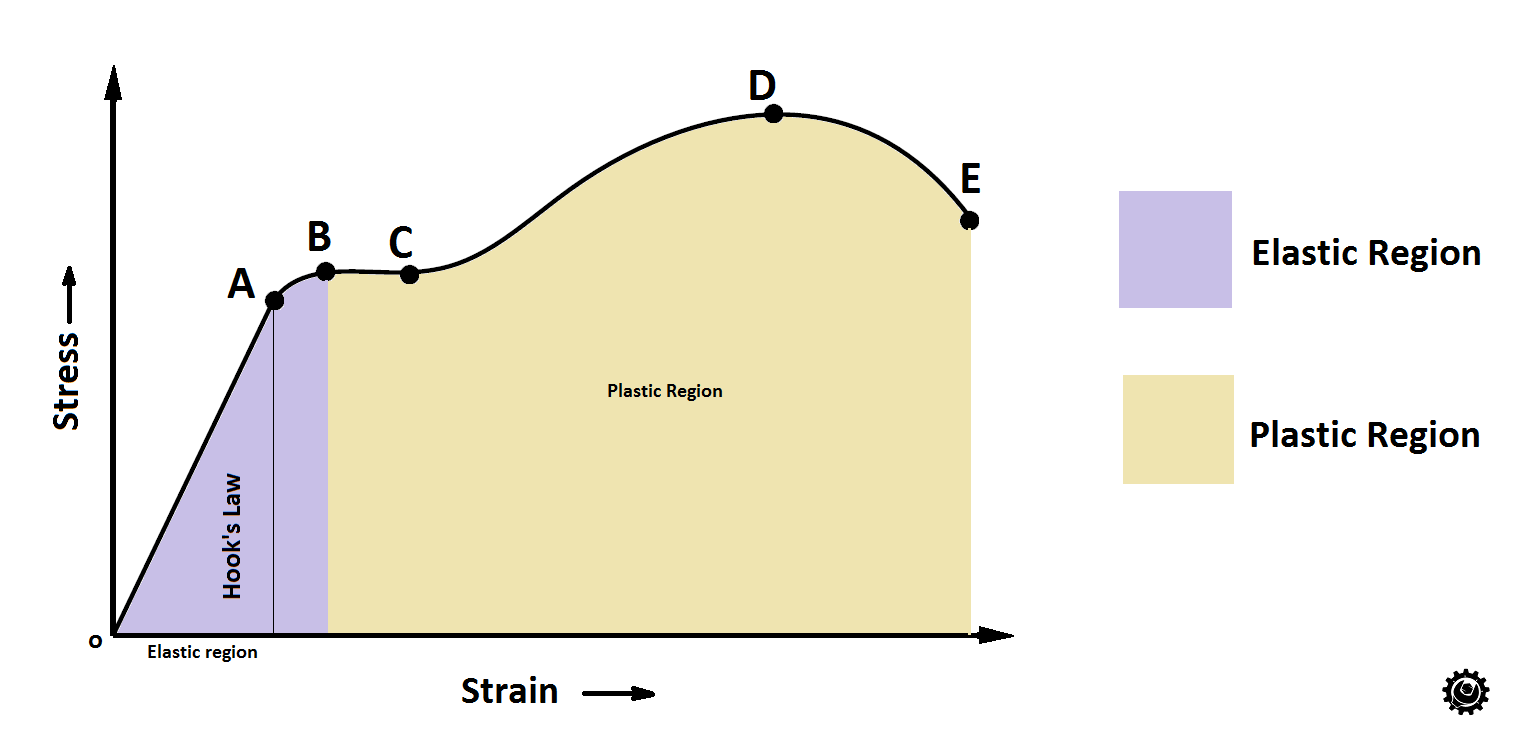
\includegraphics[width=0.9\textwidth]{pictures/stress-strain-curve-001.png}
        \caption{Stress vs. Strain. Note that the linear part of the graph represents a Hookean material that follows Hook's law.}
    \end{figure}
\end{frame}

\begin{frame}{Beyond 1D: The World of Multidimensional Stress and Strain}
    \begin{itemize}
        \item While the 1D case provides a basic understanding of stress and strain, real-world problems often involve multidimensional loading and deformation.
        \item In higher dimensions, stress and strain become tensor quantities, meaning they have both magnitude and multiple directions.
        \item This complexity arises from the fact that forces can act on a body in various directions, and the material can deform in multiple ways.
        \item To fully describe the state of stress and strain in a multidimensional setting, we need to introduce the concepts of stress and strain tensors.
        \item These tensors capture the complex interplay of forces and deformations in multiple directions, providing a more complete picture of material behavior.
    \end{itemize}
\end{frame}

\begin{frame}{Introduction to Tensors}
    \begin{itemize}
        \item Tensors are mathematical objects that generalize scalars, vectors, and matrices.
        \item They are essential tools for describing physical quantities that have both magnitude and multiple directions, such as stress, strain, and the moment of inertia.
        \item Tensors are represented by arrays of numbers, where the number of indices indicates the order of the tensor.
        \begin{itemize}
            \item Scalar: 0th-order tensor (magnitude only)
            \item Vector: 1st-order tensor (magnitude and one direction)
            \item Matrix: 2nd-order tensor (magnitude and two directions)
        \end{itemize}
    \end{itemize}
\end{frame}

\begin{frame}{Tensor Notation}
    \begin{itemize}
        \item Tensors are often represented using index notation, where subscripts indicate the components of the tensor.
        \item For example, the components of a vector $\mathbf{v}$ can be represented as $v_i$, where $i$ can take on values 1, 2, or 3 in three-dimensional space.
        \item Similarly, the components of a matrix $\mathbf{A}$ can be represented as $A_{ij}$, where $i$ and $j$ can each take on values 1, 2, or 3.
    \end{itemize}
\end{frame}

\begin{frame}{Tensor Operations}
    \begin{itemize}
        \item Tensors can be added, subtracted, and multiplied by scalars, just like vectors and matrices.
        \item They can also be multiplied together using the tensor product, which combines two tensors to form a higher-order tensor.
        \item Other important tensor operations include the dot product and the cross product, which are generalizations of the corresponding vector operations.
    \end{itemize}
\end{frame}

\begin{frame}{Tensor Product: A Deeper Dive - Part 1}
    \begin{itemize}
        \item The tensor product, denoted by $\otimes$, is a fundamental operation that combines two tensors to create a new tensor with a higher order.
        \item It's a powerful tool for representing complex relationships between quantities with multiple directions.
    \end{itemize}
\end{frame}

\begin{frame}{Tensor Product: A Deeper Dive - Part 2}
    \begin{itemize}
        \item Given a tensor $\mathbf{A}$ of order $m$ and a tensor $\mathbf{B}$ of order $n$, their tensor product $\mathbf{A} \otimes \mathbf{B}$ is a tensor of order $m + n$.
        \item This means the resulting tensor has $m + n$ indices, representing its dimensionality.
    \end{itemize}
\end{frame}

\begin{frame}{Tensor Product: A Deeper Dive - Part 3}
    \begin{itemize}
        \item The components of the tensor product are calculated by multiplying each component of the first tensor with each component of the second tensor.
        \item This can be expressed mathematically as:
        \begin{equation*}
        (\mathbf{A} \otimes \mathbf{B})_{i_1 i_2... i_m j_1 j_2... j_n} = A_{i_1 i_2... i_m} B_{j_1 j_2... j_n}
        \end{equation*}
    \end{itemize}
\end{frame}

\begin{frame}{Tensor Product: A Deeper Dive - Part 4}
    \begin{itemize}
        \item Let's break down the notation:
        \begin{itemize}
            \item $(\mathbf{A} \otimes \mathbf{B})_{i_1 i_2... i_m j_1 j_2... j_n}$ represents a component of the resulting tensor product.
            \item $A_{i_1 i_2... i_m}$ represents a component of the first tensor $\mathbf{A}$.
            \item $B_{j_1 j_2... j_n}$ represents a component of the second tensor $\mathbf{B}$.
        \end{itemize}
    \end{itemize}
\end{frame}

\begin{frame}{Tensor Product Example - Part 1}
\begin{itemize}
\item Consider two vectors:
\begin{align*}
\mathbf{a} &= \begin{bmatrix} 1 \\ 2 \\ 3 \end{bmatrix} \\
\mathbf{b} &= \begin{bmatrix} 4 \\ 5 \\ 6 \end{bmatrix}
\end{align*}
\item Their tensor product, denoted by $\mathbf{a} \otimes \mathbf{b}$, results in a second-order tensor (a matrix). 
\end{itemize}
\end{frame}

\begin{frame}{Tensor Product Example - Part 2}
\begin{itemize}
\item To compute the tensor product, we multiply each component of the first vector $\mathbf{a}$ with the entire second vector $\mathbf{b}$:
\begin{align*}
\mathbf{a} \otimes \mathbf{b} &= \begin{bmatrix} 1 \\ 2 \\ 3 \end{bmatrix} \otimes \begin{bmatrix} 4 \\ 5 \\ 6 \end{bmatrix} \\
&= \begin{bmatrix} 1 \cdot \begin{bmatrix} 4 \\ 5 \\ 6 \end{bmatrix} \\ 2 \cdot \begin{bmatrix} 4 \\ 5 \\ 6 \end{bmatrix} \\ 3 \cdot \begin{bmatrix} 4 \\ 5 \\ 6 \end{bmatrix} \end{bmatrix} 
\end{align*}
\end{itemize}
\end{frame}

\begin{frame}{Tensor Product Example - Part 3}
\begin{itemize}
\item Performing the scalar multiplication:
\begin{align*}
\mathbf{a} \otimes \mathbf{b} &= \begin{bmatrix} 1 \cdot \begin{bmatrix} 4 \\ 5 \\ 6 \end{bmatrix} \\ 2 \cdot \begin{bmatrix} 4 \\ 5 \\ 6 \end{bmatrix} \\ 3 \cdot \begin{bmatrix} 4 \\ 5 \\ 6 \end{bmatrix} \end{bmatrix} \\
&= \begin{bmatrix} \begin{bmatrix} 4 \\ 5 \\ 6 \end{bmatrix} \\ \begin{bmatrix} 8 \\ 10 \\ 12 \end{bmatrix} \\ \begin{bmatrix} 12 \\ 15 \\ 18 \end{bmatrix} \end{bmatrix}
\end{align*}
\end{itemize}
\end{frame}

\begin{frame}{Tensor Product Example - Part 4}
\begin{itemize}
\item Combining the resulting vectors into a matrix:
\begin{align*}
\mathbf{a} \otimes \mathbf{b} &= \begin{bmatrix} \begin{bmatrix} 4 \\ 5 \\ 6 \end{bmatrix} \\ \begin{bmatrix} 8 \\ 10 \\ 12 \end{bmatrix} \\ \begin{bmatrix} 12 \\ 15 \\ 18 \end{bmatrix} \end{bmatrix} \\
&= \begin{bmatrix} 4 & 5 & 6 \\ 8 & 10 & 12 \\ 12 & 15 & 18 \end{bmatrix}
\end{align*}
\end{itemize}
\end{frame}

\begin{frame}{Examples of Tensors in Mechanics}
    \begin{itemize}
        \item Stress tensor: Describes the distribution of internal forces within a deformable body.
        \item Strain tensor: Measures the deformation of a body.
        \item Moment of inertia tensor: Describes the distribution of mass in a rigid body and its resistance to rotational acceleration.
        \item Piezoelectric tensor: Relates the electric polarization of a material to the applied stress or strain.
    \end{itemize}
\end{frame}

\begin{frame}{Stress: Introduction}
    \begin{itemize}
        \item Stress is a measure of the internal force acting per unit area within a deformable body.
        \item It is a tensor quantity, meaning it has both magnitude and direction.
        \item The units of stress are typically Pascals (Pa) or pounds per square inch (psi).
        \item There are different types of stress, including normal stress (acting perpendicular to a surface) and shear stress (acting parallel to a surface).
    \end{itemize}
\end{frame}

\begin{frame}{Stress: Mathematical Definition}
    \begin{itemize}
        \item Stress is mathematically represented by the Cauchy stress tensor ($\boldsymbol{\sigma}$).
        \item It is defined as:
        \begin{equation*}
            \boldsymbol{\sigma} = \frac{\mathbf{F}}{A}
        \end{equation*}
        where:
        \begin{itemize}
            \item $\mathbf{F}$ is the force acting on a surface.
            \item $A$ is the area of the surface.
        \end{itemize}
        \item The Cauchy stress tensor describes the force acting per unit area at a point within the body.
    \end{itemize}
\end{frame}

\begin{frame}{Cauchy Stress Tensor: Fundamentals}
    \begin{itemize}
        \item The Cauchy stress tensor ($\boldsymbol{\sigma}$) is a fundamental concept in continuum mechanics that fully describes the state of stress at a point within a material.
        \item It is a second-order tensor, meaning it has both magnitude and two directions associated with it.
        \item The components of the Cauchy stress tensor represent the forces acting on the faces of an infinitesimally small cube of material surrounding the point.
    \end{itemize}
\end{frame}

\begin{frame}{Cauchy Stress Tensor: Matrix Representation}
    \begin{itemize}
        \item To visualize the Cauchy stress tensor, consider an infinitesimal cube of material surrounding a point.
        \item The stress components acting on the faces of this cube can be represented by a matrix:
        \begin{equation*}
            \boldsymbol{\sigma} = \begin{bmatrix} \sigma_{xx} & \sigma_{xy} & \sigma_{xz} \\ \sigma_{yx} & \sigma_{yy} & \sigma_{yz} \\ \sigma_{zx} & \sigma_{zy} & \sigma_{zz} \end{bmatrix}
        \end{equation*}
        \item The diagonal elements ($\sigma_{xx}$, $\sigma_{yy}$, $\sigma_{zz}$) represent the normal stresses acting on the faces perpendicular to the x, y, and z directions, respectively.
        \item The off-diagonal elements ($\sigma_{xy}$, $\sigma_{xz}$, etc.) represent the shear stresses acting on the faces.
        \item For example, $\sigma_{xy}$ represents the shear stress acting on the face perpendicular to the x-axis in the y-direction.
    \end{itemize}
\end{frame}

\begin{frame}{Cauchy Stress Tensor: Normal and Shear Stresses}
    \begin{itemize}
        \item The Cauchy stress tensor can be decomposed into normal and shear stress components.
        \item Normal stresses act perpendicular to the faces of the infinitesimal cube.
        \item Shear stresses act parallel to the faces of the infinitesimal cube.
    \end{itemize}
    \begin{figure}
        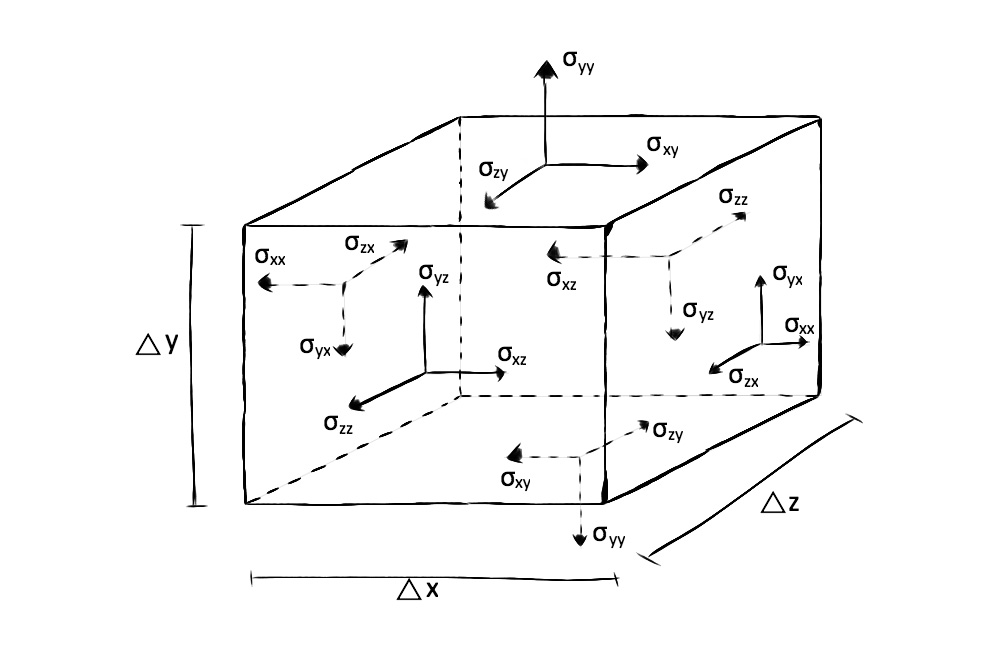
\includegraphics[width=0.5\textwidth]{pictures/moment-balance-cube.jpg}
        \caption{Shear stress acting on a cube.}
    \end{figure}
\end{frame}

\begin{frame}{Cauchy Stress Tensor: Importance}
    \begin{itemize}
        \item The Cauchy stress tensor is crucial for understanding and predicting the behavior of materials under various loading conditions.
    \end{itemize}
\end{frame}


\begin{frame}{Strain}
    \begin{itemize}
        \item Strain is a measure of the deformation of a solid body.
        \item It is a dimensionless quantity, typically expressed as a percentage or a fraction.
        \item There are different types of strain, including normal strain and shear strain.
    \end{itemize}
\end{frame}

\begin{frame}{Strain: A Mathematical Perspective - Part 1}
    \begin{itemize}
        \item Strain is a measure of the deformation of a body, quantifying how much it has stretched or compressed.
        \item It is a tensor quantity, meaning it has both magnitude and direction.
        \item Strain is often represented by the Green-Lagrange strain tensor (E), which is defined as:
        \begin{equation*}
        E = \frac{1}{2} (F^T F - I)
        \end{equation*}
        where:
        \begin{itemize}
            \item F is the deformation gradient tensor
            \item $F^T$ is the transpose of F
            \item I is the identity tensor
        \end{itemize}
    \end{itemize}
\end{frame}

\begin{frame}{Deformation Gradient Tensor}
    \begin{itemize}
        \item The deformation gradient tensor (F) is a fundamental concept in solid mechanics that describes how a body deforms.
        \item It maps the position of a point in the undeformed configuration to its corresponding position in the deformed configuration.
        \item Mathematically, F is defined as the derivative of the deformation map:
        \begin{equation*}
        F = \frac{\partial \mathbf{x}}{\partial \mathbf{X}}
        \end{equation*}
        where $\mathbf{x}$ is the position vector of a point in the deformed configuration and $\mathbf{X}$ is its position vector in the undeformed configuration.
        \item F is a second-order tensor, meaning it has both magnitude and direction.
        \item It can be used to calculate various measures of deformation, such as strain and rotation.
    \end{itemize}
\end{frame}

\begin{frame}{Derivative of the Deformation Map}
    \begin{itemize}
        \item The deformation map, denoted by $\phi$, describes how points in a body move from their initial positions ($\mathbf{X}$) in the undeformed configuration to their final positions ($\mathbf{x}$) in the deformed configuration.
        \item Mathematically, the deformation map is expressed as:
        \begin{equation*}
        \mathbf{x} = \phi(\mathbf{X})
        \end{equation*}
        \item The derivative of the deformation map, denoted by $\frac{\partial \mathbf{x}}{\partial \mathbf{X}}$ or $\nabla \mathbf{x}$, quantifies how the deformation changes with respect to the initial position.
        \item This derivative is a second-order tensor called the deformation gradient tensor (F).
        \item The deformation gradient tensor captures both the stretching and rotation of material elements during deformation.
        \item It plays a crucial role in calculating strain measures and relating stress measures between the undeformed and deformed configurations.
    \end{itemize}
\end{frame}

\begin{frame}{Stress and Strain}
    \begin{figure}
        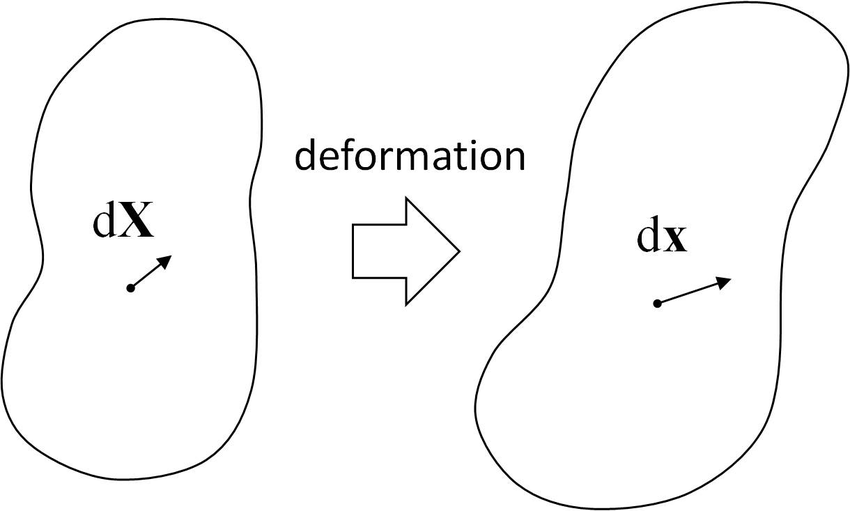
\includegraphics[width=0.9\textwidth]{pictures/Conceptual-diagram-of-deformation-gradient-tensor.png}
        \caption{Conceptual diagram of deformation gradient tensor.}
    \end{figure}
\end{frame}

\begin{frame}{Calculating the Derivative of the Deformation Map - Part 1}
    \begin{itemize}
        \item The derivative of the deformation map, denoted as $\frac{\partial \mathbf{x}}{\partial \mathbf{X}}$, quantifies how the current position $\mathbf{x}$ of a material point changes with respect to its initial position $\mathbf{X}$.
        \item This derivative is a second-order tensor called the deformation gradient tensor, often denoted by $F$.
    \end{itemize}
\end{frame}

\begin{frame}{Calculating the Derivative of the Deformation Map - Part 2}
    \begin{itemize}
        \item To calculate this derivative, we can use the following formula:
        \begin{equation*}
        F = \frac{\partial \mathbf{x}}{\partial \mathbf{X}} = \begin{bmatrix} \frac{\partial x_1}{\partial X_1} & \frac{\partial x_1}{\partial X_2} & \frac{\partial x_1}{\partial X_3} \\ \frac{\partial x_2}{\partial X_1} & \frac{\partial x_2}{\partial X_2} & \frac{\partial x_2}{\partial X_3} \\ \frac{\partial x_3}{\partial X_1} & \frac{\partial x_3}{\partial X_2} & \frac{\partial x_3}{\partial X_3} \end{bmatrix}
        \end{equation*}
        where $x_1$, $x_2$, and $x_3$ are the components of the current position vector $\mathbf{x}$, and $X_1$, $X_2$, and $X_3$ are the components of the initial position vector $\mathbf{X}$.
    \end{itemize}
\end{frame}

\begin{frame}{Calculating the Derivative of the Deformation Map - Part 3}
    \begin{itemize}
        \item Each component of the deformation gradient tensor represents the rate of change of a component of the current position with respect to a component of the initial position.
        \item This tensor provides valuable information about the local deformation, including stretching, rotation, and shearing.
    \end{itemize}
\end{frame}

\begin{frame}{Strain: A Mathematical Perspective - Part 2}
    \begin{itemize}
        \item The Green-Lagrange strain tensor measures the change in the squared length of a material line element due to deformation.
        \item For small deformations, the Green-Lagrange strain tensor can be approximated by the infinitesimal strain tensor:
        \begin{equation*}
        \epsilon = \frac{1}{2} (\nabla \mathbf{u} + (\nabla \mathbf{u})^T)
        \end{equation*}
        where $\mathbf{u}$ is the displacement vector.
    \end{itemize}
\end{frame}

\begin{frame}{Constitutive Law}
    \begin{itemize}
        \item The constitutive law of a material relates stress and strain.
        \item It describes the material's response to external forces.
        \item Different materials have different constitutive laws.
    \end{itemize}
\end{frame}

\begin{frame}{Hookean Elasticity}
    \begin{itemize}
        \item Hooke's law describes the linear elastic behavior of materials.
        \item It states that the stress is proportional to the strain:
        \begin{equation*}
            \sigma = E \epsilon
        \end{equation*}
        where $\sigma$ is the stress, $E$ is the Young's modulus, and $\epsilon$ is the strain.
        \item This law is valid for small deformations of many materials, such as metals and plastics.
    \end{itemize}
\end{frame}



\begin{frame}{Constitutive Law for a Neo-Hookean Material - Part 1}
\begin{itemize}
\item A neo-Hookean material is a type of hyperelastic material that exhibits nonlinear elastic behavior.
\item Its constitutive law relates the stress and strain in the material through a strain energy density function.
\item The strain energy density function for a neo-Hookean material is given by:
\begin{equation*}
W = \frac{\mu}{2} (I_1 - 3) + \frac{\lambda}{2} (J - 1)^2
\end{equation*}
where:
\begin{itemize}
\item $W$ is the strain energy density function
\item $\mu$ is the shear modulus
\item $\lambda$ is the bulk modulus
\item $I_1$ is the first invariant of the right Cauchy-Green deformation tensor
\item $J$ is the determinant of the deformation gradient tensor
\end{itemize}
\end{itemize}
\end{frame}

\begin{frame}{First Invariant of the Right Cauchy-Green Deformation Tensor}
\begin{itemize}
\item The right Cauchy-Green deformation tensor (C) describes the deformation of a material in terms of how line elements change their lengths and orientations. It's defined as:
\begin{equation*}
C = F^T F
\end{equation*}
where F is the deformation gradient tensor.
\item The first invariant ($I_1$) of C is a scalar quantity that measures the change in the square of the length of an infinitesimal line element due to deformation.
\item Mathematically, $I_1$ is the trace of C:
\begin{equation*}
I_1 = tr(C)
\end{equation*}
\item For a 3D deformation, $I_1$ can be expressed in terms of the principal stretches ($\lambda_1$, $\lambda_2$, $\lambda_3$), which represent the stretch ratios along the principal axes of deformation:
\begin{equation*}
I_1 = \lambda_1^2 + \lambda_2^2 + \lambda_3^2
\end{equation*}
\end{itemize}
\end{frame}

\begin{frame}{Determinant of the Deformation Gradient Tensor}
\begin{itemize}
\item The determinant of the deformation gradient tensor, denoted by $J$, is a scalar quantity that measures the local change in volume due to deformation.
\item Mathematically, $J$ is calculated as the determinant of the matrix representation of the deformation gradient tensor ($F$):
\begin{equation*}
J = \det(F)
\end{equation*}
\item Interpretation of $J$:
\begin{itemize}
\item $J > 1$: The volume at the point has increased.
\item $J < 1$: The volume at the point has decreased.
\item $J = 1$: The volume at the point has remained constant (isochoric deformation).
\end{itemize}
\item $J$ is used in various calculations in solid mechanics, such as:
\begin{itemize}
\item Relating stress measures between the deformed and undeformed configurations.
\item Calculating the strain energy density function for hyperelastic materials.
\item Ensuring mass conservation in incompressible materials.
\end{itemize}
\end{itemize}
\end{frame}

\begin{frame}{First Piola-Kirchhoff Stress}
\begin{itemize}
\item The first Piola-Kirchhoff stress tensor is a measure of the force acting per unit area in the undeformed configuration of a solid body.
\item It is related to the Cauchy stress tensor (the stress in the deformed configuration) by the deformation gradient.
\item The first Piola-Kirchhoff stress is often used in the formulation of the finite element method for solid mechanics.
\end{itemize}
\end{frame}

\begin{frame}{Calculating the First Piola-Kirchhoff Stress Tensor}
\begin{itemize}
\item The first Piola-Kirchhoff stress tensor (P) is a measure of the force acting per unit area in the undeformed configuration of a solid body.
\item It is related to the Cauchy stress tensor ($\boldsymbol{\sigma}$) by the following equation:
\begin{equation*}
P = J \boldsymbol{\sigma} F^{-T}
\end{equation*}
where J is the determinant of the deformation gradient tensor (F) and $F^{-T}$ is the inverse transpose of F.
\item Alternatively, P can be expressed in terms of the derivative of the strain energy density function (W) with respect to the deformation gradient:
\begin{equation*}
P = \frac{\partial W}{\partial F}
\end{equation*}
\item The choice of the equation depends on the specific constitutive law of the material.
\end{itemize}
\end{frame}

\begin{frame}{Constitutive Law for a Neo-Hookean Material - Part 2}
\begin{itemize}
\item The constitutive law can be expressed in terms of the first Piola-Kirchhoff stress tensor ($P$) and the deformation gradient tensor ($F$):
\begin{equation*}
P = \frac{\partial W}{\partial F} = \mu (F - F^{-T}) + \lambda J (J - 1) F^{-T}
\end{equation*}
\item This constitutive law is often used to model the behavior of rubber-like materials and biological tissues.
\end{itemize}
\end{frame}

\begin{frame}{Deriving the First Piola-Kirchhoff Stress Tensor - Part 1}
\begin{itemize}
\item Recall that the strain energy density function for a neo-Hookean material is:
\begin{equation*}
W = \frac{\mu}{2} (I_1 - 3) + \frac{\lambda}{2} (J - 1)^2
\end{equation*}
\item To find the first Piola-Kirchhoff stress tensor, we take the derivative of W with respect to the deformation gradient tensor F:
\begin{equation*}
\mathbf{P} = \frac{\partial W}{\partial \mathbf{F}}
\end{equation*}
\end{itemize}
\end{frame}

\begin{frame}{Deriving the First Piola-Kirchhoff Stress Tensor - Part 2}
\begin{itemize}
\item Using the chain rule, we can break down the derivative as follows:
\begin{align*}
\mathbf{P} &= \frac{\partial W}{\partial \mathbf{F}} \\
&= \frac{\partial}{\partial \mathbf{F}} \left[ \frac{\mu}{2} (I_1 - 3) + \frac{\lambda}{2} (J - 1)^2 \right] \\
&= \frac{\mu}{2} \frac{\partial I_1}{\partial \mathbf{F}} + \lambda (J - 1) \frac{\partial J}{\partial \mathbf{F}}
\end{align*}
\end{itemize}
\end{frame}

\begin{frame}{Deriving the First Piola-Kirchhoff Stress Tensor - Part 3}
\begin{itemize}
\item Now, we need the following identities:
\begin{align*}
\frac{\partial I_1}{\partial \mathbf{F}} &= 2 \mathbf{F} \\
\frac{\partial J}{\partial \mathbf{F}} &= J \mathbf{F}^{-T}
\end{align*}
\item Substituting these identities into the previous equation, we get:
\begin{align*}
\mathbf{P} &= \frac{\mu}{2} \cdot 2 \mathbf{F} + \lambda (J - 1) \cdot J \mathbf{F}^{-T} \\
&= \mu \mathbf{F} + \lambda J (J - 1) \mathbf{F}^{-T}
\end{align*}
\end{itemize}
\end{frame}

\begin{frame}{Equations of Motion for an Elastic Body}
    \begin{itemize}
        \item The equations of motion for an elastic body describe the dynamic behavior of the body under the influence of external forces.
        \item They are typically expressed in terms of the displacement field, the stress tensor, and the body force density.
        \item The equations of motion can be derived from the principle of virtual work or the principle of least action.
    \end{itemize}
\end{frame}

\begin{frame}{Equations of Motion for an Elastic Body - Part 1}

    \begin{itemize}
        \item The equations of motion for an elastic body describe how the body deforms and moves under the influence of external forces.
        \item These equations are typically derived from the conservation of linear momentum and angular momentum.
        \item For a continuous elastic body, the equations of motion can be expressed in the following general form:
        \begin{equation*}
        \rho \frac{\partial^2 \mathbf{u}}{\partial t^2} = \nabla \cdot \boldsymbol{\sigma} + \mathbf{f}
        \end{equation*}
        where:
        \begin{itemize}
            \item $\rho$ is the density of the material
            \item $\mathbf{u}$ is the displacement vector
            \item $t$ is time
        \end{itemize}
    \end{itemize}
\end{frame}

\begin{frame}{Equations of Motion for an Elastic Body - Part 2}
    \begin{itemize}
        \item The equation of motion from the previous slide is:
        \begin{equation*}
        \rho \frac{\partial^2 \mathbf{u}}{\partial t^2} = \nabla \cdot \boldsymbol{\sigma} + \mathbf{f}
        \end{equation*}
        Continuing the explanation of the terms:
        \begin{itemize}
            \item $\nabla \cdot$ is the divergence operator
            \item $\boldsymbol{\sigma}$ is the Cauchy stress tensor
            \item $\mathbf{f}$ is the body force vector (e.g., gravity)
        \end{itemize}
        \item This equation states that the acceleration of a point in the body is proportional to the sum of the internal stresses and external forces acting on it.
        \item The specific form of the equations of motion depends on the constitutive law of the material and the type of analysis being performed (e.g., static, dynamic).
    \end{itemize}
\end{frame}



\begin{frame}{Supporting Figures}
    \begin{figure}
        \includegraphics[width=0.8\textwidth]{solid_mechanics_concepts.png}
        \caption{Illustration of solid mechanics concepts.}
    \end{figure}
\end{frame}

\begin{frame}{Glossary of Terms}
  \begin{description}
    \item[Stress] A measure of the force acting per unit area within a deformable body.
    \item[Tensor] A mathematical object that describes a multilinear relationship between sets of algebraic objects related to a vector space.
    \item[Cauchy Stress Tensor ($\boldsymbol{\sigma}$)] A second-order tensor that describes the state of stress at a point within a material.
    \item[Normal Stress] Stress acting perpendicular to a surface.
    \item[Shear Stress] Stress acting parallel to a surface.
    \item[Pascal (Pa)] The SI unit of pressure or stress, equal to one newton per square meter.
    \item[Pound per Square Inch (psi)] A unit of pressure or stress in the imperial and US customary systems.
    \item[Continuum Mechanics] The branch of mechanics that deals with the analysis of the kinematics and mechanical behavior of materials modeled as a continuous mass rather than as discrete particles.
  \end{description}
\end{frame}

\end{document}